\chapter{ITERATOR}

Pattern comportamentale usato per accedere ai contenuti di un oggetto aggregato senza esporne la rappresentazione interna e fornisce un modo uniforme per 
attraversare tale collezione, indipendentemente dal tipo di collezione o dalla sua struttura sottostante.

Supponiamo di avere una classe scuola, avente una collezione di studenti.

Se restituissimo la collezione con un classico getter pubblico, esporremmo troppi dettagli interni ai client permettendogli di manipolare direttamente la collezione.

Se un giorno decidessi di cambiare l'implementazione della collezione, i client ne risentiranno.

Un getter protected non migliorerebbe la situazione in quanto ai client esterni basterebbe estendere la nostra classe per usare quel getter.

Invece facendo tornare un iteratore, non forniamo un punto di accesso alla collezione, infatti se decidessi di passare da collezione ad un set, non avrei problemi 
di compilazione (col getter classico li avrei avuti).

\textbf{N.B.} Un iteratore non conosce il numero di elementi di un aggregato, può solamente attraversarli.

\section{Struttura}

\begin{figure}[H]
    \centering
    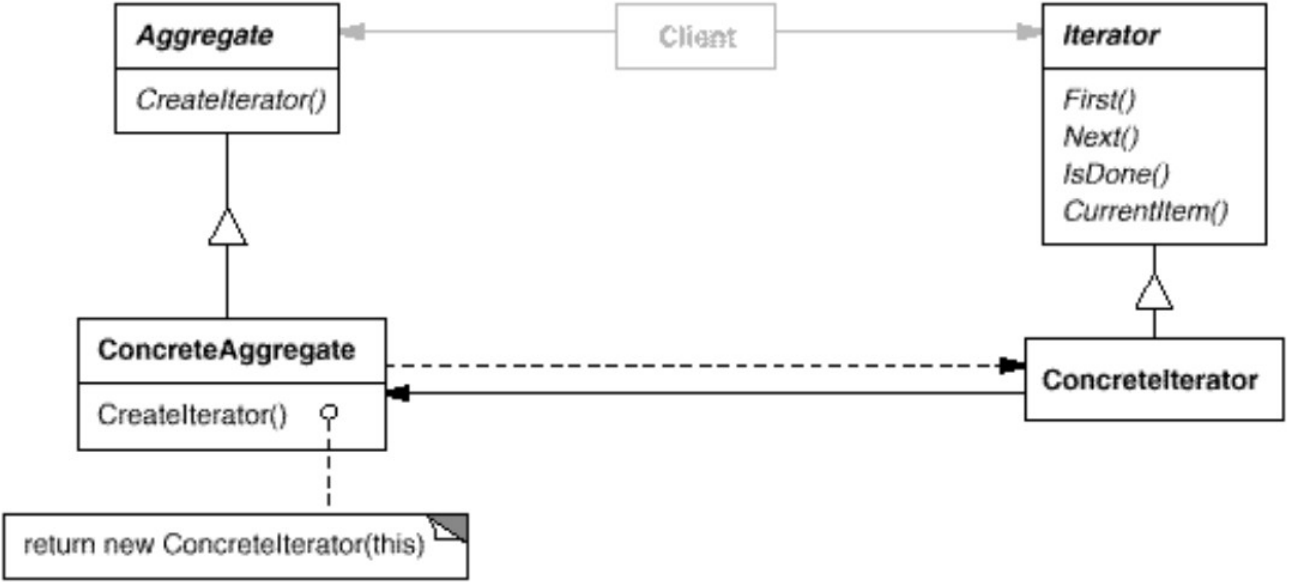
\includegraphics[width=0.5\linewidth]{../../immagini/iterator/struttura_visitor}
\end{figure}

\textbf{Iterator} definisce l'interfaccia per attraversare gli elementi e offre metodi come hasNext() per verificare se ci sono altri elementi da attraversare e next()
per ottenere l'elemento successivo.

\textbf{Aggregate} è l'interfaccia o la classe astratta che rappresenta la collezione di oggetti. 
Fornisce un metodo per ottenere un iteratore che può essere utilizzato per attraversare gli elementi.

\textbf{ConcreteIterator} implementa Iterator e tiene traccia, durante l’attraversamento, dell’oggetto corrente e deve essere in grado di calcolare l’elemento successivo.
Per questo ha un riferimento all’aggregato concreto.

\textbf{ConcreteAggregate}  implementa Aggregate e crea un opportuno ConcreteIterator.

\section{Iterator vs Stream}

Possono sembrare simili.

Gli stream sono più astratti e possono essere parallelizzati.
Si basano su un approccio dichiarativo, permettono facilmente di filtrare, raggruppare, partizionare e gestiscono completamente in automatico l’attraversamento dell’aggregato.

Gli iteratori sono molto più semplici, permettono di attraversare un aggregato un elemento alla volta, sono per loro stessa natura sequenziali ma richiedono che hasNext e next siano usati correttamente insieme.